\documentclass{article}[]
\usepackage{epsfig}
\usepackage{psfig}
\usepackage{graphicx}
\usepackage{url}
\usepackage{times}
\usepackage[colorlinks,linkcolor=red,anchorcolor=blue,citecolor=green]{hyperref}

\begin{document}

\title{{\bf Title of Project}\\ }

\author{Wang Xin\\ \vspace{0.5cm}\\
 10302010023}

\date{}
\maketitle
\begin{abstract}
Abstract goes here
\end{abstract}

\section{Introduction}
\label{intro}
Introduction here

\subsection{Subsection}

Use citations like this \cite{Mckay:2010} and reference elements such as
Figs.~\ref{code:ant20} and \ref{fig:trail}, Eq.~\ref{eq1}, and Table
\ref{table:params}.

\begin{figure}
\centering
\begin{verbatim}
move();

or

if(food_ahead == 1){
        move();
else{
        move();
}
\end{verbatim}
\caption{Example solution at Energy 20.}%
\label{code:ant20}%
\end{figure}

\begin{figure}
\centering
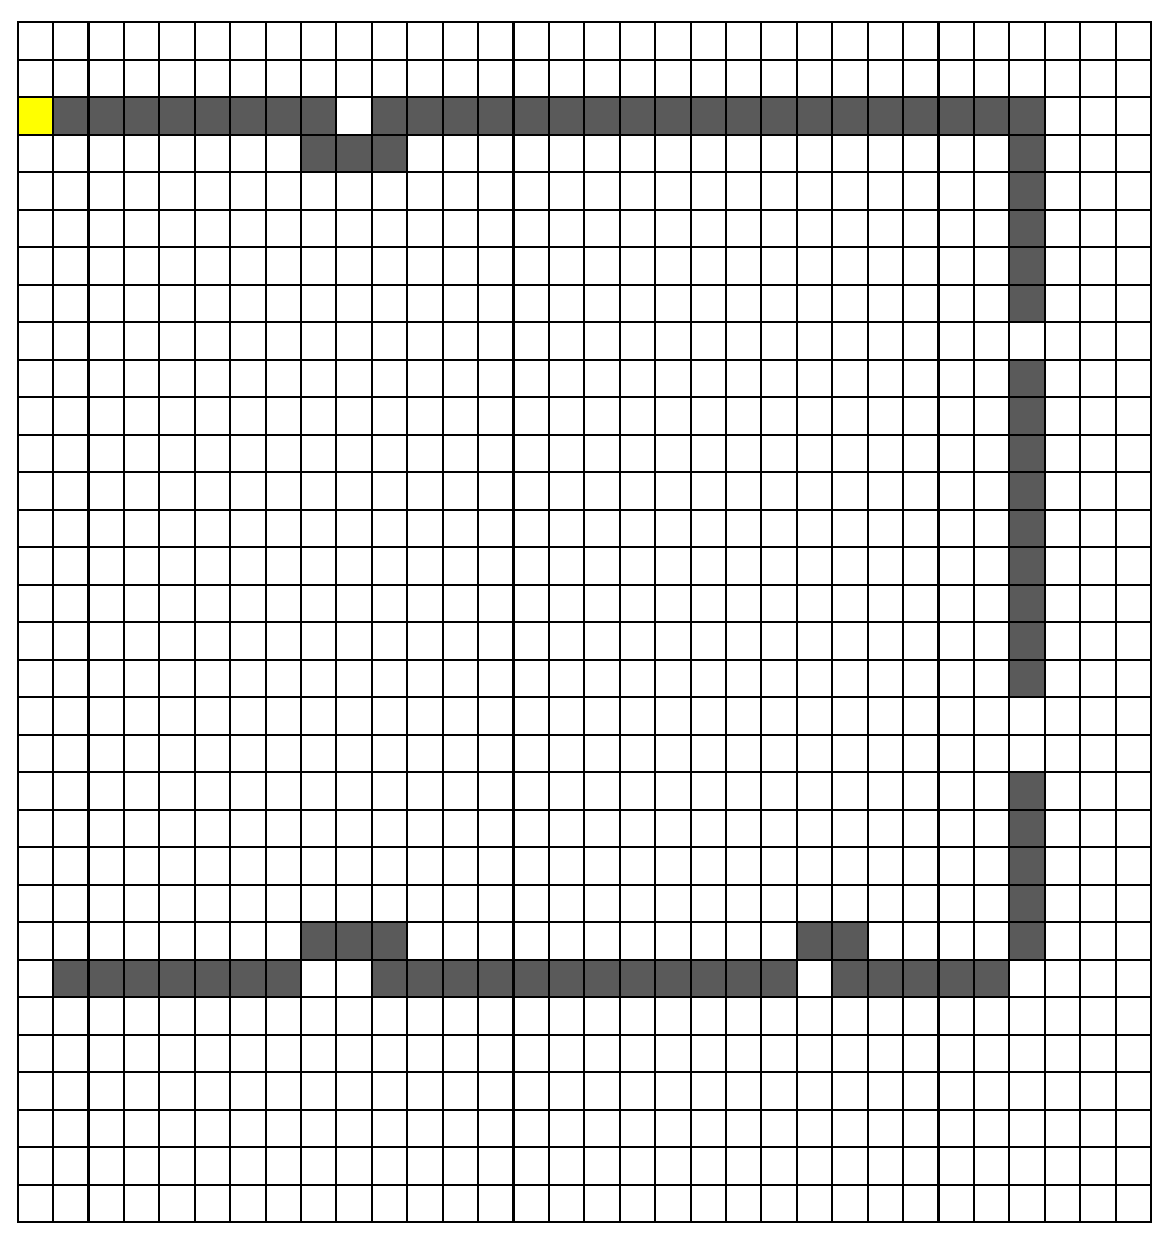
\includegraphics[width=0.50\textwidth]{trail.pdf}
\caption{Dynamic Ant Trail.}
\label{fig:trail}
\end{figure}

\begin{equation} New\ Node\ =\ Codon\ value\ \%\ Number\ of\ rules\ for\ NT
\label{eq1}
\end{equation}

\begin{table}
\caption{Parameter settings adopted on all problems examined} % title of Table
\centering      % used for centering table
\begin{tabular}{l|c}  % centered columns
\hline                      %inserts double horizontal lines
{\bf Parameter}&{\bf Value}\\
%heading
\hline                    % inserts single horizontal line
Total Evaluations & 100,000\\
Evals per cycle & 500, 2500, 5000, 10,000\\
Generations & 200\\
Population size & 500\\
Replacement strategy & Generational with elitism (10\%)\\
Selection & Tournament size=5\\
Mutation probability & 0.02 (integer mutation)\\
Crossover probability & 0.9 (variable single point)\\
Initial chromosome length & 100 codons (random init)\\
\hline     %inserts single line
\end{tabular}
\label{table:params}
 \end{table}

\section{Compiling}

If you are using a GUI, this document should compile automatically. Otherwise,
you can either use pdflatex or latex and dvi2ps to compile your report, along
with bibtex to process your bibliography file.

%ACKNOWLEDGEMENTS are optional
\section{Acknowledgements}
People you might want to acknowledge.

\bibliographystyle{abbrv}
\bibliography{biblio}

\end{document}

